\section{subhalo342447における$\mathrm{[X/Fe]} > 0$について}

図\ref{fig:fe10}に示すように,X $=$ Ne, O, Mg, Siとして$\mathrm{[X/Fe]} > 0$がいえる.このようなXをアルファ($\alpha$)元素という.中性子数と陽子数が偶数で等しく,$\alpha$粒子(\ce{^{4}He})の集まりと見なせることから,この名前で呼ばれている.Feよりもアルファ($\alpha$)元素が多いということは,アルファ($\alpha$)元素の生成元される重力崩壊型超新星爆発(II型超新星爆発)に由来するものと考えられる.

II型超新星の中心部では核融合反応が進行し,アルファ($\alpha$)元素を生成する.核融合のエネルギーと重力が平衡状態であったのが,鉄まで生成されると平衡状態が崩れ,収縮を始める.中心核は中性子の縮退圧と重力が枯渇すると急停止し,上層は中心核によって反跳し衝撃波が発生する.ゆえに大量のアルファ($\alpha$)元素を宇宙空間にばらまくことになる.

\section{アウトフローと太陽組成比との関係}

アウトフローが観測されたsubhalo342447は図\ref{fig:abundanceprofile342447}に示したように,R/R$_{200} < 0.1$において太陽組成の2倍近くFe, O, Mg, Siなどの元素が観測された.一方でアウトフローが観測されなかったsubhalo388544やsubhalo421555はR/R$_{200} < 0.1$において太陽組成程度であることが観測された(図\ref{fig:2radicalprofile}).

このようなことからアウトフローと太陽組成には何らかの因果関係がある可能性がある.

\section{subhalo342447の「へこみ」と温度分布の高温部}

図\ref{fig:fe10}において$0.1<\text{R/R}_{200} < 0.5$で他の部分と組成が異なる「へこみ」が観測されたことに加え,図\ref{fig:atemp}の右側で,R/R$_{200} < 0.1$においては\SI{e6}{K}以上の高温ガスが確認できたことから,subhalo342447が現在の状態になるまでに,他のsubhaloと衝突をし,そのsubhaloの組成の一部を取り込んだ可能性が考えられる.

\begin{figure}[htbp]
	\centering
	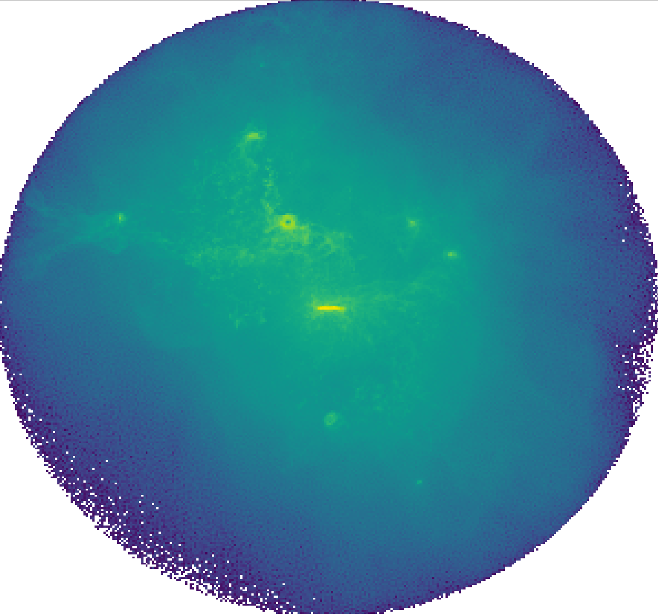
\includegraphics[width=0.6\linewidth]{pic/virial3}
	\captionsetup{width=0.9\linewidth}
	\caption{subhalo342447をedge-onにした状態で中心にとり,ビリアル半径の3倍を表示.濃淡は対数で質量を表す.}
	\label{fig:virial3}
\end{figure}

また図\ref{fig:virial3}に示すようにsubhalo342447の周囲に別のsubhaloが観測され,ガスの散乱具合も衝突後のような状態となっている.このようなことから衝突した可能性は非常に高いと考えられる.